% Section 2: Materials and Methods (with Table 1, model inputs). Follows paper/outline.md.
% All result numbers and design constants are \Num... macros from paper/numbers.tex (generated by paper/R/export_numbers.R).
% No \documentclass: this file is \input into the MDPI main file.
\section{Materials and Methods}
\label{sec:methods}

The valuation chain has five steps (Figure~\ref{fig:fig1_design}). A tool profile, defined by five technical inputs, is simulated in a stochastic breeding program (Layer 1). The simulated genetic gain is calibrated to realized progress in common bean and converted into adoption-weighted value over a grid of economic states (Layer 2). The resulting net present value (NPV) is attributed to its inputs and entered into a decision analysis. The tool enters the model only through its technical inputs, and we do not model its image-analysis algorithm. Three meta-analyses of published studies supply the ranges and central values of the tool inputs and the calibration target (Section~\ref{sec:ma}). Throughout, ``accuracy'' denotes the inverse of the error variance of the phenotype used for selection and is distinct from the selection accuracy $r$ of the breeder's equation.

\begin{figure}[H]
\centering
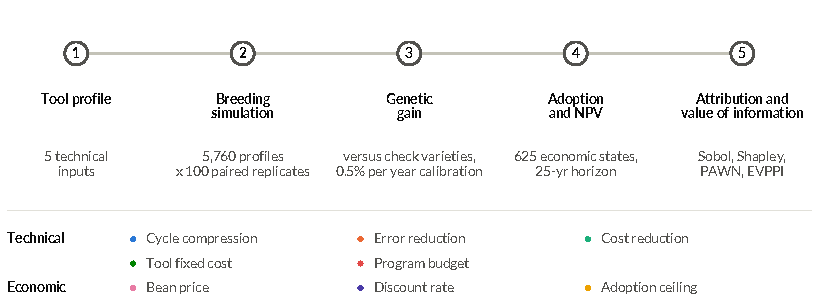
\includegraphics[width=\linewidth]{figures/fig1_design}
\caption{Study design. Each tool profile (five technical inputs) is simulated in a stochastic common-bean breeding program; its genetic gain over the check varieties is calibrated to realized progress, valued through variety adoption and discounting over the economic states, and attributed to its inputs. The colors identify the model inputs in all later figures.\label{fig:fig1_design}}
\end{figure}

\subsection{Case and Breeding Pipeline}
\label{sec:case}

The case is a public common-bean program in East Africa with a four-stage testing pipeline and a \NumCfgCycleYears{}-year cycle from cross to release. The stages are an observation nursery (ON), a preliminary yield trial (PYT), an advanced yield trial (AYT) and a national performance trial (NPT). The cycle length is an assumption of the model. A dry-bean simulation study used an eight-year cycle \cite{Lin2023Simulations}, and a CGIAR review notes that the path from a program decision to a widely grown variety, which includes adoption, rarely takes less than ten years \cite{Kholova2021Pursuit}. In this model $L$ is the time from cross to release, not the parent-recycling interval of the breeder's equation, and the adoption lag after release is modeled separately in Layer 2. Each cycle starts with \NumCfgNcrosses crosses among founders, each yielding \NumCfgNprogeny F1 plants, followed by \NumCfgNssd generations of single-seed descent to F5. The resulting F5 lines form the pool that enters the ON. Table~\ref{tab:inputs} lists lines, replicates, environments and selected fraction for each stage. These stage sizes are assumptions in the style of pipelines of the Pan-Africa Bean Research Alliance (PABRA), not values reported by a single source. The NPT selects \NumCfgNreleased lines for release.

Yield is simulated as a single additive polygenic trait on the \NumCfgNchr{} chromosomes of the common-bean genome \cite{Schmutz2014Reference}. The founder population has \NumCfgNfounders individuals, \NumCfgSegSites segregating sites per chromosome and \NumCfgQTLperChr quantitative trait loci (QTL) per chromosome, and the QTL number is an assumption. Mean yield is \NumCfgMeanYield{} kg/ha, consistent in order of magnitude with national average yields reported for African bean-growing countries \cite{Beebe2013Phenotyping} and with the average reported for Tanzania \cite{Hillocks2006Phaseolus}. The additive genetic standard deviation of the founders is \NumCfgSigmaA{} kg/ha, an assumption whose absolute scale the calibration removes (Section~\ref{sec:calibration}). Plot-level heritability of yield is \NumCfgHtwoYield{}, and the correlation that parameterizes genotype-by-environment interaction (GxE) between on-station environments is \NumCfgGxEOnstation. No source reports either value for this pipeline, so both are assumptions that a robustness block varies (Section~\ref{sec:inputs}).

\subsection{Layer 1: Stochastic Breeding Simulation}
\label{sec:layer1}

Each breeding cycle was simulated in AlphaSimR \cite{Gaynor2020Alphasimr}, with founder haplotypes from its coalescent simulator, for a manual program and a tool program in every replicate. Both programs share one founder population per replicate. Random founder pairs, drawn without replacement for each cross, produce F1 plants that are advanced to F5 by selfing. The four stages then apply truncation selection on phenotype, and a random subsample enters a stage when more lines are available than its size. AlphaSimR serves the strategic design of CGIAR-type programs with replicated stochastic runs \cite{Seck2024Stochastic,Gorjanc2018Optimal,FritscheNeto2023Improving}. Haplotype generation is not controlled by the R random-number seed, so a single replicate cannot be replayed in isolation.

Each stage selects on one phenotype per line, whose error variance gives the heritability of a genotype mean over the stage's replicates and environments. Let $\sigma^2_A$ be the genetic variance of the selection target and let GxE variance be parameterized as $\sigma^2_{GE} = (1-\rho_{GE})\,\sigma^2_A$, which is the parameterization implemented in the simulation. Then
\begin{equation}
h^2_{\mathrm{eff}} = \left[\, 1 + \frac{1-\rho_{GE}}{e} + \frac{1-h^2}{h^2\, r\, e} \,\right]^{-1},
\label{eq:heff}
\end{equation}
where $h^2$ is plot-level heritability, $r$ the number of replicates and $e$ the number of environments. Under the common variance-component definition of the genetic correlation between environments, $\rho = \sigma^2_A/(\sigma^2_A+\sigma^2_{GE})$, the same GxE variance corresponds to $\rho = 1/(2-\rho_{GE})$, so $\rho_{GE}$ is a parameter of this model and not a measured genetic correlation. The error variance of the single phenotype is
\begin{equation}
\sigma^2_{\varepsilon} = V_{\mathrm{ref}} \left( \frac{1}{h^2_{\mathrm{eff}}} - 1 \right),
\label{eq:vare}
\end{equation}
where $V_{\mathrm{ref}}$ is the genetic variance of the F5 pool entering the ON, computed once per program run. Plot error therefore stays constant across stages while selection depletes genetic variance, so realized heritability falls from stage to stage, whereas $h^2_{\mathrm{eff}}$ keeps its meaning on the F5-line basis. The tool's error reduction $\delta$ scales the single-plot error variance by $(1-\delta)$ before averaging over replicates and environments. With the single-plot error variance normalized to one, $\sigma^2_A = h^2/(1-h^2)$, and the tool program replaces $h^2$ in Equation~(\ref{eq:heff}) by
\begin{equation}
h^2_{\mathrm{tool}} = \frac{\sigma^2_A}{\sigma^2_A + (1-\delta)}.
\label{eq:htool}
\end{equation}
The genotype-by-environment term is unchanged by the tool, and $\delta$ may be negative for a tool noisier than manual scoring.

Genetic gain is the mean true genetic value of the released lines minus that of the check varieties, taken as the top $k$ founders, with $k$ equal to the number of released lines. The checks stand in for the elite varieties that farmers already grow. The gain over the founder mean is kept as a secondary output. For the manual program it averages \NumDGvsBaseTradPerCycle{} kg/ha per cycle across profiles, against \NumDGtradPerCycle{} kg/ha over the checks (both uncalibrated), so the check baseline is the more conservative reference. Both programs use common random numbers. Within a replicate they start from the same founder population, and the generator is re-seeded with the same pipeline seed immediately before each program runs. Crosses and generation advance are therefore identical, and noise largely cancels in the paired difference. Annual gain is the per-cycle gain divided by the cycle length, $L$ for the manual program and $L-c$ for the tool program with cycle compression $c$. A tool's advantage is expressed as the per-cycle uplift $u = 100\,\bar{D}/\bar{G}_{\mathrm{man}}$ (mean paired difference over mean manual gain), the annual uplift $100\,[(1+u/100)\,L/(L-c) - 1]$, and the equivalent compression $L - L/(1+u/100)$, the years of compression that raise annual gain by the same percentage as $u$. Figure~\ref{fig:fig2_time_beats_accuracy}b applies the last conversion to the mean per-cycle uplift of each robustness setting, averaged over its cost-reduction and compression levels, so the exchange rate includes the effect of cost reduction.

Both programs spend the same total budget per cycle, so a cheaper plot or a fixed tool cost changes how many lines and environments can be tested. Trial cost is the sum over stages of lines $\times$ environments $\times$ replicates $\times$ cost per plot, plus the tool fixed cost, which is zero for the manual program. The manual cost per plot is USD \NumCfgCostPerPlot, an assumption that also appears in \cite{Juliana2018Integrating} and is consistent in order of magnitude with East African costing \cite{Das2025Costing}. The tool's cost per plot is the manual cost multiplied by $(1-\text{cost reduction})$. A grid search varies PYT size from \NumCfgPYTmin{} to \NumCfgPYTmax{} lines in steps of \NumCfgPYTstep{} and PYT environments from one to \NumCfgPYTenvMax{}. The ON size is \NumCfgONmult{} times the PYT size, capped at \NumCfgONcap{} lines and at the F5 pool (crosses times progeny per cross), and ON plots are single-replicate and single-environment. The AYT and NPT sizes stay at the values in Table~\ref{tab:inputs}. Among the allocations that fit the budget, the search selects the maximizer of the breeder's-equation approximation of annual gain \cite{Cobb2019Enhancing}, $\hat{G} = L^{-1}\sum_{s} i_s \sqrt{h^2_{\mathrm{eff},s}}\,\sigma_A$, where $i_s$ is the selection intensity implied by the selected fraction of stage $s$. The allocation is chosen once per program and tool profile and used in every replicate. It trades the number of entries against replication \cite{Lorenz2013Resource}.

\subsection{Tool Inputs and Sweep Design}
\label{sec:inputs}

A tool profile is defined by five technical inputs: measurement-error reduction, whole-plot cost reduction, cycle compression, tool fixed cost and program budget (Table~\ref{tab:inputs}). Error reduction is the fractional reduction of single-plot error variance, and cost reduction is the fractional reduction of whole-plot cost. The simulated trait is yield, which a smartphone tool does not measure, because grain is harvested and weighed. No source we read shows how an image-based measure would lower the error variance of plot yield, for example by covariate adjustment with image-derived stand counts, and that pathway is untested here. Error reduction is therefore an effective reduction in the error variance of the selection phenotype, and the meta-analytic evidence for it concerns trait-level measurement error (Section~\ref{sec:ma}). It is not a measured property of yield recording.

Cycle compression is the number of years by which the tool shortens the breeding cycle. It leaves the simulated selection unchanged, because stage sizes, replicates and error variance do not depend on it, and it acts through the cycle length that divides gain and through the timing of release and spending in Layer 2. The simulation therefore treats compression as a scenario and does not model how a tool would achieve it. A tool could shorten the cycle only by bringing forward a selection decision, for example when stage data arrive early enough to recycle parents sooner \cite{Seck2024Stochastic}. Where beans are grown in two seasons per year, as in the bimodal-rainfall areas of Rwanda, Uganda and parts of Tanzania, the smallest such step is half a year; parts of the region, including most of Ethiopia and southern Tanzania, have a single bean season \cite{Katungi2018Effect,Jha2023Characterizing,Hillocks2006Phaseolus}. The main grid uses whole years from zero to \NumCfgCycMax{} because Layer 2 runs on an annual step, and a seasonal check covers zero, \NumCfgSeasonMid{} and one year (Section~\ref{sec:robust}). We found no study that measured how far a phenotyping tool shortens a breeding cycle. Precedents exist for other cycle-shortening technologies in dry bean, maize and rice \cite{Lin2023Simulations,Chaingeni2025More,Katiyar2026Unified}. Fixed cost (equipment and training) and budget are in USD per cycle, and the fixed cost is paid from within the budget. The evidence-based profile has an error reduction of \NumCfgErrRedCentral{}\% and a cost reduction of \NumCfgCostRedCentral{}\% (Section~\ref{sec:ma}). The error reduction is the median of the heritability-pair route (\NumERhtwoMedian\%) rounded to the nearest ten percent, whereas route T1 and the converted route T2 give negative medians, so this central value is at the favorable end of the evidence. The lower end of the fixed-cost range lies above reported hardware costs \cite{Mwanje2026Digital,Whan2014Grainscan}, and its upper end assumes training and data management. The budget grid lies above the operating cost per cycle reported for single national programs, USD \NumNatCostMin{} to \NumNatCostMax{} for maize pipelines in Uganda, Zambia and Zimbabwe and rice pipelines in four countries \cite{Das2025Costing,Katiyar2026Unified}, and it brackets the average operating cost of public breeding programs in the United States reported in \cite{Chaingeni2025More}, which cites a 2020 survey. We therefore model a regional breeding network: the pipeline pools the evaluation capacity of several national programs, and the grid spans the combined budget of roughly \NumNetProgMin{} to \NumNetProgMax{} national programs at these costs. Bean area is summed over the same six countries, so benefits and costs refer to the same scope. The cost anchors come from maize and rice and stand in for bean, so the network budget remains an assumption; because the budget barely moves the attribution of value (Section~\ref{sec:res_measure}), the conclusions do not depend on where in this range a real network lies.

\begin{table}[H]
\caption{Model inputs, explored values, central values and sources. ``Assumption'' marks values set by the authors that no cited source reports; each is explored in the sensitivity analysis or removed by the calibration.\label{tab:inputs}}
\begin{adjustwidth}{-\extralength}{0cm}
\footnotesize
\setlength{\tabcolsep}{3pt}
\begin{tabularx}{\fulllength}{>{\raggedright\arraybackslash}p{3.9cm}>{\raggedright\arraybackslash}p{2.0cm}>{\raggedright\arraybackslash}p{3.2cm}>{\raggedright\arraybackslash}p{2.6cm}>{\raggedright\arraybackslash}X}
\toprule
\textbf{Input} & \textbf{Unit} & \textbf{Explored values} & \textbf{Central or baseline} & \textbf{Source or status}\\
\midrule
\multicolumn{5}{l}{\textit{Technical inputs of the tool}}\\
Measurement-error reduction & \% of plot error variance & \NumCfgErrRedRange & \NumCfgErrRedCentral & Heritability-pair route of MA2, rounded (Section~\ref{sec:ma}); compatible with zero; effective reduction in selection error\\
Whole-plot cost reduction & \% of whole-plot cost & \NumCfgCostRedRange & \NumCfgCostRedCentral & MA3 time saving times data-capture share of plot cost \cite{Reynolds2019Costefficient}; upper bound on the saving from data capture alone\\
Cycle compression & Years & \NumCfgCycRange & \NumCfgCycCompCentral & Scenario; no measured effect found; precedents \cite{Lin2023Simulations,Chaingeni2025More,Katiyar2026Unified}\\
Tool fixed cost & USD per cycle & \NumCfgFixCostRange & \NumCfgFixCostCentral & Assumption; lower end above reported hardware costs \cite{Mwanje2026Digital,Whan2014Grainscan}\\
Program budget & USD per cycle & \NumCfgBudgetRange & \NumCfgBudgetCentral & Assumption: regional network of about \NumNetProgMin{}--\NumNetProgMax{} national programs \cite{Das2025Costing,Katiyar2026Unified}\\
\midrule
\multicolumn{5}{l}{\textit{Genetic and pipeline inputs}}\\
Plot-level heritability of yield & Ratio & \NumCfgRobHtwoLevels & \NumCfgHtwoYield{} & Assumption\\
GxE parameter $\rho_{GE}$ between on-station environments & Ratio & \NumCfgRobGxELevels & \NumCfgGxEOnstation & Assumption; $\sigma^2_{GE}=(1-\rho_{GE})\sigma^2_A$\\
Additive genetic standard deviation & kg/ha & Not varied & \NumCfgSigmaA{} & Assumption; scale removed by calibration\\
Chromosomes; founders; segregating sites and QTL per chromosome & Count & Not varied & \NumCfgNchr; \NumCfgNfounders; \NumCfgSegSites; \NumCfgQTLperChr & Chromosomes \cite{Schmutz2014Reference}; founders, sites and QTL are assumptions\\
Mean yield & kg/ha & Not varied & \NumCfgMeanYield{} & Order of magnitude consistent with \cite{Beebe2013Phenotyping,Hillocks2006Phaseolus}\\
Cycle length & Years & Not varied & \NumCfgCycleYears{} & Assumption; an eight-year dry-bean cycle is used in \cite{Lin2023Simulations}\\
Crosses per cycle; progeny per cross; selfing generations & Count & Not varied & \NumCfgNcrosses; \NumCfgNprogeny; \NumCfgNssd & Assumption\\
ON: lines; replicates; environments; selected \% & Count; \% & Lines optimized under the budget (Section~\ref{sec:layer1}) & \NumCfgStageONLines; \NumCfgStageONReps; \NumCfgStageONEnvs; \NumCfgStageONSelFrac{} & Assumption; PABRA-style pipeline\\
PYT: lines; replicates; environments; selected \% & Count; \% & Lines and environments optimized under the budget & \NumCfgStagePYTLines; \NumCfgStagePYTReps; \NumCfgStagePYTEnvs; \NumCfgStagePYTSelFrac{} & Assumption; PABRA-style pipeline\\
AYT: lines; replicates; environments; selected \% & Count; \% & Not varied & \NumCfgStageAYTLines; \NumCfgStageAYTReps; \NumCfgStageAYTEnvs; \NumCfgStageAYTSelFrac{} & Assumption; PABRA-style pipeline\\
NPT: lines; replicates; environments; selected \% & Count; \% & Not varied & \NumCfgStageNPTLines; \NumCfgStageNPTReps; \NumCfgStageNPTEnvs; \NumCfgStageNPTSelFrac{} & Assumption; PABRA-style pipeline\\
Manual cost per plot & USD & Not varied & \NumCfgCostPerPlot & Assumption that also appears in \cite{Juliana2018Integrating}; order of magnitude consistent with \cite{Das2025Costing}\\
\midrule
\multicolumn{5}{l}{\textit{Calibration and economic inputs}}\\
Realized gain target & \% of mean yield per year & Not varied in the main analysis; \NumCfgTargetLow{} and \NumCfgTargetHigh{} in robustness scenarios & \NumGainTargetPct{} & MA1 (Section~\ref{sec:ma})\\
Bean price & USD/kg & \NumCfgPriceRange & \NumBasePrice{} & Assumption informed by the mean and range of farm-gate prices in Uganda \cite{Jjagwe2022Role}\\
Discount rate & \% & \NumCfgDiscRange & \NumBaseDisc{} & Rates in practice \cite{Harberger2015Musings,Groom2022Future}\\
Adoption ceiling & \% of bean area & \NumCfgAdoptRange & \NumBaseAdopt{}\textsuperscript{a} & Levels consistent with \cite{Alene2019Measuring,Spielman2019Policy}; a modeling choice\\
Bean area & Million ha & \NumCfgAreaRange & \NumBaseArea{} & Brackets FAOSTAT area harvested \cite{FAO2025FAOSTATQCL}\\
Logistic rate; midpoint & Per year; years & Not varied in the main analysis; rate \NumCfgKLow{} and \NumCfgKMid{} in robustness scenarios & \NumCfgDiffK; \NumCfgDiffMid & Assumption; observed pace \cite{Alene2019Measuring}\\
Evaluation horizon & Years & Not varied in the main analysis; \NumCfgHorizonLong{} in a robustness scenario & \NumCfgHorizon{} & Common in ex ante work \cite{Staver2020ExAnte}\\
Tool running cost (net-value scenarios only) & Million USD per year & \NumCfgRunCostLow, \NumCfgRunCostMid{} and \NumCfgRunCostHigh & Not in the main NPV & Assumption; the order of magnitude of a global system is ``a few million USD per year'' \cite{Lasdun2024Participatory}\\
\bottomrule
\end{tabularx}
\end{adjustwidth}
\noindent{\footnotesize{\textsuperscript{a} The configured central adoption ceiling lies midway between two grid levels, and the baseline state takes the lower level.}}
\end{table}

The main grid and two extension blocks form one full factorial design of \NumNcellsOK{} tool profiles (\NumNgridTech{} combinations of error reduction, cost reduction, fixed cost and budget at each of four compression levels), each simulated with \NumNrepsPerCell{} paired replicates. The main grid crosses five levels of error reduction, five of cost reduction, four of cycle compression, six of fixed cost and five of budget (\NumNcellsMain). Extension A adds an error reduction of zero across eight levels of cost reduction, because the agreement evidence in MA2 is compatible with no improvement over manual scoring (\NumNcellsExtA). Extension B adds the lower whole-plot cost reductions implied by MA3 for the positive error reductions (\NumNcellsExtB). The union has six levels of error reduction and eight of cost reduction. The mean standard error of the paired per-cycle difference is \NumDGdiffSE{} kg/ha (uncalibrated). A stress block of \NumNcellsStress{} further profiles was simulated at zero compression with an error reduction of \NumCfgStressErr\%, that is, a tool noisier than manual scoring, at the lowest and the central cost reduction, the central fixed cost and three budgets; because compression leaves the selection unchanged, Layer 2 reuses these gains at every compression level. The stress block is not part of the main lookup table. Simulations ran on the Rorqual cluster of Calcul Qu\'ebec and the Digital Research Alliance of Canada.

Because no source reports plot-level heritability or the on-station GxE parameter for this pipeline, a separate robustness block varies both on a reduced tool grid. It crosses three levels of heritability (\NumCfgRobHtwoLevels) and three of the GxE parameter (\NumCfgRobGxELevels) with five levels of error reduction (zero to the maximum), three of cost reduction and four of cycle compression, at the baseline fixed cost and budget. It comprises \NumNcellsRobust profiles with \NumNrepsPerCell{} replicates each. The block feeds Figures~\ref{fig:fig2_time_beats_accuracy}b and \ref{fig:fig3_gain_ceiling}c only and is not part of the economic lookup table.

\subsection{Calibration of Simulated Gain to Realized Progress}
\label{sec:calibration}

We rescaled simulated gain by one common factor so that the manual program's mean annual gain equals realized progress in common-bean breeding. Averaged over all profiles, the simulated manual program gains \NumDGtradPerYear{} kg/ha per year over the checks, or \NumDGtradPctPerYearRaw\% of mean yield per year, which exceeds the realized rate. The target is \NumGainTargetPct{}\% per year of the mean yield of \NumCfgMeanYield{} kg/ha, the pooled realized gain of common-bean programs in MA1 (Section~\ref{sec:ma}). Three of the four programs in MA1 are Brazilian, the East African PABRA estimates alone are about 0.5\% per year \cite{Amongi2023Gain}, and the confidence interval of the pooled estimate reaches zero. Public programs that serve smallholders realize well under one percent annually \cite{Cobb2019Enhancing}. The factor of \NumGainScale{} multiplies the manual gain, the tool gain and the paired difference of every profile, and gives a calibrated manual gain of \NumDGtradPerYearCal{} kg/ha per year. Relative per-cycle uplifts are unchanged by this step, and money values shrink. NPV is not proportional to the factor, because the program budget in the cash flow is not rescaled. Gain is proportional to the additive genetic standard deviation in the breeder's-equation approximation of this model, so the common factor is equivalent to setting that standard deviation to \NumGainScale{} of its assumed value. A calibration through lower plot-level heritability or a lower GxE parameter would instead change relative uplifts, but the simulated manual program gains \NumRobManualGainPctMin{} to \NumRobManualGainPctMax{} percent of mean yield per year across the robustness block, at least \NumRobManualGainFoldMin{} times the target, so heritability within the explored range cannot close the gap. If real programs gain slowly because their effective heritability is below the explored range, accuracy would carry more value than we report, and we did not run that case, which needs Layer 1 simulations at lower heritability. We tested the calibration target at \NumCfgTargetLow{} and \NumCfgTargetHigh{}\% per year (Section~\ref{sec:robust}). Era-trial rates reflect decades of overlapping cycles, whereas the simulation covers one cycle, which adds to the uncertainty of the target.

\subsection{Layer 2: Adoption, Net Present Value and Equivalent Annual Value}
\label{sec:layer2}

The value of the tool is the net present value of its incremental cash flow over the manual program across a \NumCfgHorizon{}-year horizon $H$ (years zero to $H$). Let $L_j$ be the cycle length of program $j$, with $L_{\mathrm{man}} = L$ and $L_{\mathrm{tool}} = L-c$. Each program spends its budget evenly over the $L_j$ years of its cycle, so a shorter cycle spends the same budget sooner. The tool's fixed cost acts through the Layer 1 allocation and is not an additional cash flow, and the main NPV excludes the cost of developing, hosting and supporting the tool (Section~\ref{sec:robust} adds it as a scenario). Release occurs at the end of the cycle, in year $L_j$. From release, the yield advantage of the released lines over the check varieties builds at the annual gain $g_j = G_j/L_j$ until it equals the per-cycle gain $G_j$ after $L_j$ years, and then stays at $G_j$. The ramp is a modeling simplification: it lets the advantage build over one cycle length, as successive releases from overlapping cycles would, and then credits no further cycles. The benefit of program $j$ in year $t \geq L_j$ is
\begin{equation}
B^{j}_t = g_j\,\min(t-L_j+1,\,L_j)\; p\; a(t-L_j)\; A,
\label{eq:benefit}
\end{equation}
where $p$ is the bean price, $a(\cdot)$ the adoption rate and $A$ the bean area. The spending $C^{j}_t$ equals the budget divided by $L_j$ in years before release and zero afterwards. With $r$ the discount rate,
\begin{equation}
\mathrm{NPV} = \sum_{t=0}^{H} \frac{\left(B^{\mathrm{tool}}_t - B^{\mathrm{man}}_t\right) - \left(C^{\mathrm{tool}}_t - C^{\mathrm{man}}_t\right)}{(1+r)^{t}}.
\label{eq:npv}
\end{equation}
We use NPV rather than a benefit-cost ratio, which favors underinvestment \cite{Janssen2018Costbenefit}. The gains $G$ are the calibrated means over replicates for each profile. NPV therefore varies across tool profiles and economic states but not across replicates, so Monte Carlo variation within a profile does not enter the NPV distribution.

Adoption follows a logistic curve with a ceiling, the standard form in ex ante breeding evaluations \cite{Grovermann2022Three},
\begin{equation}
a(\tau) = \frac{K}{1 + \exp\left[-k\,(\tau - \tau_{\mathrm{mid}})\right]},
\label{eq:logistic}
\end{equation}
where $\tau$ is the time since release, $K$ the adoption ceiling, $k$ the rate and $\tau_{\mathrm{mid}}$ the midpoint. The ceiling is swept. The rate (\NumCfgDiffK) and the midpoint (\NumCfgDiffMid) are fixed assumptions in the main analysis. The assumed rate implies a faster gain in area than the roughly one percentage point per year observed for improved beans \cite{Alene2019Measuring}, so slower rates are tested in the robustness scenarios. The ceiling levels are consistent with a modern-variety share of about one third of bean area \cite{Alene2019Measuring} and a similar mean across African crops, which is reported secondhand \cite{Spielman2019Policy}.

Each tool profile was valued at every state of the full factorial of five levels of each of four economic inputs: bean price, discount rate, adoption ceiling and bean area. This design gives \NumNlookupRows{} profile-state combinations. The price levels span the mean farm-gate prices reported for Uganda (0.37 and 0.51 USD per kg) and extend above the observed maximum of 1.14 USD per kg, whereas the lowest level lies above the observed minimum of 0.20 USD per kg \cite{Jjagwe2022Role}. The discount-rate levels bracket the rates that Global South governments and development banks use \cite{Harberger2015Musings,Groom2022Future}. The area levels range from \NumCfgAreaRange{} million ha. They bracket the dry-bean area harvested in \NumFaoYearFrom{}--\NumFaoYearTo{}, which was \NumFaoSixMin{}--\NumFaoSixMax{} million ha summed over Uganda, Kenya, Tanzania, Rwanda, Burundi and Ethiopia and \NumFaoEAMin{}--\NumFaoEAMax{} million ha for the FAOSTAT region of Eastern Africa \cite{FAO2025FAOSTATQCL}. Area harvested counts land once per season, so in two-season areas it exceeds the physical bean area; the annual benefit per hectare in Layer 2 is defined on the same basis. The baseline state takes the grid point nearest the configured central values: a price of \NumBasePrice{} USD/kg, a discount rate of \NumBaseDisc{}\%, an adoption ceiling of \NumBaseAdopt{}\% and an area of \NumBaseArea{} million ha. The stressed state combines the lowest price, the highest discount rate, the lowest ceiling and the smallest area. In that state we also computed, for every pair of levels of two tool inputs, the median NPV over the remaining tool inputs (the break-even marginals). The equivalent annual value (EAV) per hectare converts NPV into a level annual stream over the horizon,
\begin{equation}
\mathrm{EAV} = \frac{\mathrm{NPV}\; r}{\left[1-(1+r)^{-H}\right] A}.
\label{eq:eav}
\end{equation}
Multiplying EAV by the area gives the level annual cost that the program could carry before NPV falls to zero, the break-even running cost.

\subsection{Global Sensitivity and Decision Analysis}
\label{sec:gsa}

The Layer 1 profiles and the economic levels form a full factorial grid. With area fixed at the baseline, the model is a table of NPV values over eight inputs (the five technical inputs plus price, discount rate and adoption ceiling), and every conditional expectation $\mathrm{E}[Y \mid X_S]$ of NPV $Y$ given a subset $S$ of inputs follows by exact averaging over the table (\NumNexactGrid{} values). All inputs take their simulated levels with equal probability, so one prior serves the variance attribution and the decision analysis. This replaces the sampling of continuous uniform inputs mapped to the nearest simulated profile, which gave the end levels half the weight of the interior levels. Area is fixed at the baseline in both analyses. First-order and total-order Sobol indices \cite{Sobol2001Global} follow from $S_i = \mathrm{Var}(\mathrm{E}[Y \mid X_i])/\mathrm{Var}(Y)$ and $S^T_i = 1 - \mathrm{Var}(\mathrm{E}[Y \mid X_{-i}])/\mathrm{Var}(Y)$. They are exact, so they carry no Monte Carlo error and no sample-size choice. A total-order index of zero is necessary and sufficient for an input to be non-influential \cite{Pianosi2016Sensitivity}. The remaining uncertainty is the noise in the Layer 1 gains. To gauge it, we added normal noise with the standard error of each profile's paired difference to the tool gain, recomputed the indices \NumBootB{} times and report the largest shift of any total-order index.

Three further measures test whether the ranking depends on the variance attribution or on input independence. Shapley effects \cite{Owen2017Shapley,Song2016Shapley,Iooss2019Shapley} were computed exactly as the average of the marginal contribution of each input over all orderings of the eight inputs, with the cost function $c(S) = \mathrm{Var}(\mathrm{E}[Y \mid X_S])$, for independent inputs and for a Gaussian copula discretized on the grid. For independent inputs, each Shapley effect must lie between the first-order and total-order indices \cite{Iooss2019Shapley}, which we verified for every input. The copula correlations are assumptions: positive for discount rate with price (correlation \NumCfgCopRhoPriceDisc), adoption ceiling with budget (\NumCfgCopRhoAdoptBudget) and compression with error reduction (\NumCfgCopRhoCycErr), and negative for cost reduction with fixed cost (\NumCfgCopRhoCostFix). The four pairs are disjoint, so the joint probability of a grid point is the product of four bivariate normal rectangle probabilities. PAWN \cite{Pianosi2015Simple} is the median Kolmogorov-Smirnov distance between the conditional distribution of NPV at each level of an input and its unconditional distribution, computed exactly on the grid. Its magnitude depends on the choice of summary statistic \cite{Puy2020Sensitivity}. Horizon-dependent total-order indices use the NPV truncated at each year from zero to \NumCfgHorizon{} with the same prior. Active subspaces \cite{Constantine2014Active} come from central finite-difference gradients at \NumCfgASN{} random points in normalized space, with a step of \NumCfgASstep{} in normalized units on each side, for the lookup mapped to the nearest simulated profile. Because that lookup is piecewise constant, a gradient differs from zero only where a step crosses a boundary between grid levels, so the eigenvalues depend on the step and on the spacing of the grid, and we use them as a qualitative check. The eigenvalues give shares of the mean squared gradient. Because each measure answers a different question, we compare rankings across measures, not magnitudes.

The expected value of perfect partial information (EVPPI) measures how much learning an input would be worth to a decision between investing in the tool and an alternative with a fixed payoff $\tau$, the hurdle \cite{Claxton2001Bayesian}. For input $X_i$,
\begin{equation}
\mathrm{EVPPI}_i(\tau) = \mathrm{E}_{X_i}\!\left[\max\left(\mathrm{E}[\mathrm{NPV}\mid X_i],\,\tau\right)\right] - \max\left(\mathrm{E}[\mathrm{NPV}],\,\tau\right).
\label{eq:evppi}
\end{equation}
We computed it exactly on the grid by conditioning on each level of each of the eight inputs, under the prior above. Three hurdles are used. The first is a multiple of the prior expected NPV (\NumEVprior{} million USD), from zero to \NumCfgHurdleMaxMult{} times that value; EVPPI peaks at the indifference hurdle $\tau = \mathrm{E}[\mathrm{NPV}]$ by construction, and no named alternative investment sets that value. The second is zero, the decision to invest in the tool or not. The third applies the zero hurdle to NPV net of an incremental annual running cost of \NumCfgRunCostLow, \NumCfgRunCostMid{} and \NumCfgRunCostHigh{} million USD paid in every year of the horizon, which makes the investment decision depend on the information. Conditioning on grid levels avoids the upward bias of nested Monte Carlo with small inner samples \cite{Brennan2007Calculating} and the regression step of single-sample estimators \cite{Strong2013Estimating,Heath2017Review}. An EVPPI above the cost of research is necessary but not sufficient for the research to be worthwhile \cite{Rothery2020Value}.

Expected NPV was also decomposed into a pessimistic corner, an optimistic corner and the remaining mixed states, over all profile-state combinations including area. The pessimistic corner has price, adoption ceiling and cycle compression at or below the lower tercile cut point of their distributions over the lookup table, and the discount rate at or above the upper cut point. With five levels per economic input and four levels of compression, this assigns the lowest two levels of price and ceiling, the highest two levels of discount rate, and zero or one year of compression to the corner. The optimistic corner is the mirror image. Because compression has four levels and none falls in the middle tercile, the remaining states form one mixed group, so three groups result. For each group we report the share of states, the mean and median NPV and the probability that NPV is negative.

\subsection{Robustness Analyses}
\label{sec:robust}

Each robustness analysis re-evaluates the exact NPV table under one changed assumption, without new Layer 1 simulation, and reports the same measures (expected NPV, total-order indices of compression and error reduction, and EVPPI at the indifference hurdle). Four analyses change the prior on cycle compression: levels zero and one year with equal weight; zero with probability \NumCfgZeroMassA{} and one to three years sharing the rest; zero with probability \NumCfgZeroMassB{} and one year with the rest; and seasonal steps of \NumCfgSeasonStep{} year with compression of zero, \NumCfgSeasonMid{} and one year, for which the gains of the four compression cells of each profile are pooled, because compression leaves selection unchanged. Five analyses change the economic structure: no ramp, so that the full per-cycle gain applies from release; recurrent cycles, in which the advantage keeps accruing each year without the cap and spending continues every year; a horizon of \NumCfgHorizonLong{} years; and adoption rates of \NumCfgKLow{} and \NumCfgKMid{}. A combination with no ramp, a rate of \NumCfgKLow{} and a horizon of \NumCfgHorizonLong{} years is also run with compression of zero or one year. Two analyses change the calibration target to \NumCfgTargetLow{} and \NumCfgTargetHigh{}\% per year. The running-cost scenarios subtract the annual cost above from the NPV. The no-ramp variant removes the faster ramp of the shorter cycle and so lowers the weight of compression. The recurrent-cycle variant credits more cycles to the shorter program and so raises it, and it bounds the simplification of the single-cycle model from the other side.

\subsection{Literature Searches and Meta-Analyses of Model Inputs}
\label{sec:ma}

Three meta-analyses grounded the model inputs. MA1 pools realized genetic gain in common bean, with other African staples as context. MA2 pools agreement between image-based or AI tools and manual references. MA3 pools time and cost savings of digital phenotyping. Candidate studies came from a federated search of OpenAlex, Semantic Scholar and Crossref that returned at most 25 records per query and source, supplemented for MA3 by direct queries of Crossref and Europe PMC. All searches ran on \NumSearchDate{}, with \NumPrismaOneQueries{}, \NumPrismaTwoQueries{} and \NumPrismaThreeQueries{} queries for MA1, MA2 and MA3 (query strings and hit counts in Supplementary Table S1). The searches identified \NumPrismaOneRecords{}, \NumPrismaTwoRecords{} and \NumPrismaThreeRecords{} records, of which \NumPrismaOneUnique{}, \NumPrismaTwoUnique{} and \NumPrismaThreeUnique{} remained after removing duplicates by DOI; reference lists and the other literature searches of this project contributed \NumPrismaOneOther{}, \NumPrismaTwoOther{} and \NumPrismaThreeOther{} further candidates. Of \NumPrismaOneSought{}, \NumPrismaTwoSought{} and \NumPrismaThreeSought{} reports sought, \NumPrismaOneAssessed{}, \NumPrismaTwoAssessed{} and \NumPrismaThreeAssessed{} were obtained legally and read in full, and \NumPrismaOneIncluded{}, \NumPrismaTwoIncluded{} and \NumPrismaThreeIncluded{} studies were included (flow diagrams in Supplementary Figure S1). Title and abstract screening was logged record by record only for MA2, where a title-keyword rule removed off-topic records; for MA1 and MA3 the number of records excluded at screening was not recorded. The MA1 pool rests on \NumMAoneKclus programs, so its prediction interval is indicative. A study entered a model only if it was marked as included, its DOI was verified against Crossref and re-checked live, and its full text had been read. Every extracted value carries its page or table locator. No formal risk-of-bias tool was applied. Table~\ref{tab:ma2appraisal} instead lists, for each MA2 effect, the crop, trait, platform, type of manual reference, unit of observation and preprint status. Some discovery queries timed out, so statements that no study was found refer to these searches only. Preprints stay in the primary sets and are removed in a sensitivity analysis. Topic searches on breeding simulation, phenotyping tools, breeding and adoption economics, and sensitivity and value-of-information methods also looked for a coupled breeding-simulation and adoption-economics valuation of a phenotyping tool, for global sensitivity analysis of a stochastic breeding simulation, and for value-of-information analysis of a breeding or phenotyping investment. We found none, and a re-run on \NumNoveltyDate{} with \NumNoveltyQueries{} queries in the federated search and in Crossref confirmed this; OpenAlex and Semantic Scholar were unavailable during the re-run because of rate limits, so it rests mainly on Crossref. The closest studies simulate phenotyping in breeding pipelines without adoption economics or value-of-information analysis \cite{Peixoto2023Simulationbased,Jahufer2021Deterministic,Lane2021High}.

All pooled estimates come from random-effects models fitted by REML in metafor, with three-level models where several effects share a program or study and Knapp-Hartung (t) intervals because the number of effects is small. For MA1, the effect is the regression slope divided by the era-trial mean, in percent of mean yield per year, with standard errors taken or derived from the source tables. For MA2, correlations were Fisher z-transformed with sampling variance $1/(n-3)$, where $n$ is the number of observation units of the effect (plots, plants, images, accessions, lines or cultivars; Table~\ref{tab:ma2appraisal}), and Spearman coefficients and square roots of $R^2$ were treated as Pearson correlations. Because the pooled correlation mixes traits, platforms and reference types with very high heterogeneity, it is descriptive, and the trait-specific estimates are the more meaningful summaries. Small-study checks (an Egger-type test, a rank test and trim-and-fill) were applied at the study level only. For MA3, the effect is the log ratio of time per unit of data, pooled without weights because no study reports a variance, so the random-effects model amounts to an unweighted t-interval, and back-transformed to a percent time reduction. We report 95\% prediction intervals next to confidence intervals, because they describe what a new program or tool might show. Sensitivity analyses used one effect per cluster, leave-one-out, exclusion of preprints and imputed standard errors. Pooled estimates are shown in Table~\ref{tab:meta}.

A tool-manual correlation does not identify error reduction, so we bounded it by three routes. Let $E = 1-\rho^2$ be the error share of a measurement, with $\rho$ its correlation with the true value, and $\mathrm{ER} = 1 - E_{\mathrm{tool}}/E_{\mathrm{manual}}$. Route T1 treats the manual reference as error-free, so that $\rho_{\mathrm{tool}}$ equals the pooled correlation. Route T2 treats the reference as a manual measure with independent errors, so that $\rho_{\mathrm{tool}}$ equals the pooled correlation divided by the correlation of manual scoring with the true value, $\rho_{\mathrm{manual}}$. The manual-reliability evidence (MA2b, three studies) contains three kinds of coefficient: correlations of a visual estimate with a digital measurement of the true severity, which estimate $\rho_{\mathrm{manual}}$ directly; correlations between two raters, which for parallel measures with independent errors equal $\rho_{\mathrm{manual}}^2$; and squared correlations between two ratings, which equal $\rho_{\mathrm{manual}}^4$. We pooled the coefficients as entered, which gives T2 as entered, and again after converting every row to $\rho_{\mathrm{manual}}$ by taking the square root of between-rater correlations and the fourth root of squared correlations, which gives T2 converted. Intra-rater repeatability also contains persistent rater bias, so the converted value is an upper bound on validity. We propagated the sampling uncertainty of the pooled correlations through T1 and both T2 variants by Monte Carlo (\NumMAtwoMCdraws{} draws) and discarded infeasible draws under T2. The third route uses heritability pairs, the ratio of noise to signal $(1-h^2)/h^2$ for image traits over manual traits. Whole-plot cost reduction is the data-capture (non-handling) share of plot cost, taken from a cost model for high-income phenotyping infrastructure and therefore an upper bound on the saving from data capture alone \cite{Reynolds2019Costefficient}, multiplied by the time saving of field handheld tools \cite{Walter2019Highthroughput,Lasdun2024Participatory}.

\subsection{Software and Reproducibility}
\label{sec:software}

The full chain from simulation summaries to every number in the text is scripted. Layer 1 was run on a computing cluster in R \NumRVersionHPC{} with AlphaSimR \NumAlphaSimRVersionHPC{} and data.table. Layer 2, the exact sensitivity and decision analyses, the robustness scenarios and the number export were run locally in R \NumRVersionLocal{} with data.table, arrow and mvtnorm. The meta-analyses ran in R \NumRVersionMA{} with metafor \NummetaforVersion{}. Figures were drawn in Python with matplotlib. A Makefile regenerates the Layer 2 outputs and the file of number macros, so every result number in the manuscript is a generated macro. The tables of meta-analysis results and the appraisal table are generated from the same files. Code and data availability: \TODO{repository URL and archive DOI}.
